\documentclass[letterpaper]{article} % DO NOT CHANGE THIS
\usepackage[submission]{aaai2027}  % DO NOT CHANGE THIS
\usepackage[hyphens]{url}  % DO NOT CHANGE THIS
\usepackage{graphicx} % DO NOT CHANGE THIS
\urlstyle{rm} % DO NOT CHANGE THIS
\def\UrlFont{\rm}  % DO NOT CHANGE THIS
\usepackage{natbib}  % DO NOT CHANGE THIS AND DO NOT ADD ANY OPTIONS TO IT
\usepackage{caption} % DO NOT CHANGE THIS AND DO NOT ADD ANY OPTIONS TO IT
\frenchspacing  % DO NOT CHANGE THIS
\usepackage{algorithm}
\usepackage{algorithmic}
\usepackage{booktabs}
\usepackage{amsmath,amssymb,amsthm}
\usepackage{multirow}

\pdfinfo{
/TemplateVersion (2027.1)
}

\setcounter{secnumdepth}{1}

% float packing: let floats fill more of each page so wide tables/figures do not orphan
\renewcommand{\topfraction}{0.92}
\renewcommand{\bottomfraction}{0.85}
\renewcommand{\textfraction}{0.08}
\renewcommand{\floatpagefraction}{0.80}
\setcounter{topnumber}{3}
\setcounter{totalnumber}{5}

\theoremstyle{plain}
\newtheorem{proposition}{Proposition}

\newcommand{\mdemph}[1]{\emph{#1}}
\newcommand{\memph}[1]{\emph{#1}}
\newcommand{\R}{\mathbb{R}}
\newcommand{\X}{\mathcal{X}}
\newcommand{\D}{\mathcal{D}}

\title{Decomposing the GP Advantage in Offline MBO}

\author{Anonymous Submission}
\affiliations{}

\begin{document}

\maketitle

\begin{abstract}
Offline model-based optimization ships a surrogate and an optimizer together and reports one number, leaving open which of the two it credits, as the subfield's own 2026 survey concedes \citep{kim2025mbosurvey}. We cross both axes under one shared protocol, three surrogate classes against three search routines, and decompose the outcome variance between them. The crossed design estimates the term a one-factor-at-a-time study cannot, and it is our strongest result: on the synthetic grid the surrogate$\times$optimizer interaction ($\eta^2_{\text{inter}}\approx0.15$ under min--max normalization) has a bootstrap interval excluding zero in all four engine corners and exceeds the optimizer main effect in eleven of twelve corner$\times$normalizer combinations, inverting only under rank normalization. A design that fixes the acquisition rule and varies only the surrogate \citep{li2024bnnsurrogates} cannot see it. The interaction also dissolves a real confusion: a small optimizer \mdemph{marginal} ($\eta^2_{\text{opt}}{=}0.038$) licenses ``optimizer choice explains little variance'' but never ``optimizer choice is arbitrary,'' because its \mdemph{conditional} effect is four to thirty-three times larger. Any $\eta^2$ headline is in turn a joint artifact of five operating-point coordinates---ensemble size $K$, pessimism $\beta$, search budget, engine corner, and the per-task normalizer---so a headline stating fewer is not reproducible, and we state all five. The instrument that exposes those coordinates is a taxonomy of five confounds specific to offline-MBO surrogate comparison, each traced to a line of the scoring path with a signed effect and a pre-registered kill criterion, of which the $\beta$--$\sigma$ criterion fired. We find no prior offline-MBO work reporting a crossed surrogate$\times$optimizer variance decomposition; Policy-Guided Gradient Search, whose Table 1 supplies our reference point, fixes the surrogate and never crosses it \citep{chemingui2024pggs}. Correcting the two \mdemph{protocol} confounds moves the surrogate effect \mdemph{up}, not down---from our decomposition of PGS's Table 1 ($\eta^2_{\text{surr}}\approx0.37$) to $0.405$ $[0.290,0.556]$, a direction we found no precedent for---though the corner intervals do not resolve at $n{=}7$ tasks, so we claim the direction, not a level, and $\eta^2_{\text{surr}}>\eta^2_{\text{opt}}$ in all twelve corner$\times$normalizer combinations. What the surrogate advantage \mdemph{is} stays open, narrowed by seven controls (Section~\ref{sec:mech}). On Design-Bench we detect no surrogate difference at this power, which at $n{=}7$ tasks is not equivalence, and matching query budgets there \mdemph{raises} the optimizer effect $1.5$ to $1.9\times$ rather than dissolving it. That the statistical model often outranks the acquisition heuristic is a decade-old doctrine we do not contest \citep{shahriari2016humanoutoftheloop}; what this design falsifies is the local premise of one recent paper \citep{chemingui2024pggs}, not any field-level belief.
\end{abstract}

% \begin{links}
%   \link{Code}{https://anonymous.4open.science/r/offline-mbo-decomposition}
% \end{links}

\section{Introduction}

Offline model-based optimization (MBO) seeks a design $x$ maximizing an expensive black-box $f$ from a fixed dataset $\D=\{(x_i,y_i)\}_{i=1}^N$, with no further queries to $f$ during search \citep{trabucco2022designbench,kim2025mbosurvey}. The dominant recipe fits a surrogate $\hat f$ and optimizes it; because optimization pushes designs into regions where $\hat f$ is unconstrained, the surrogate is typically made conservative, by a learned regularizer \citep{trabucco2021coms} or by a pessimistic acquisition such as the lower confidence bound (LCB) $\mu(x)-\beta\sigma(x)$ \citep{srinivas2010ucb}. A common intuition holds that Gaussian-process LCB (GP-LCB) beats neural-ensemble LCB at low dimension because the GP posterior is better calibrated. But the two pipelines differ in \mdemph{two} coupled factors, not one: the surrogate class (GP posterior vs.\ ensemble disagreement) and the acquisition optimizer, since GPs are usually optimized by perturbation or quasi-Newton restarts and neural surrogates by gradient ascent on $x$. Every method in this lineage ships both at once and reports one number---leaving open which of the two the number credits.

\begin{figure}[t]
\centering

\includegraphics[width=0.99\columnwidth]{figures_v3/schematic}
\caption{The design: a crossed surrogate$\times$optimizer factorial (three surrogate classes against three search routines under one shared protocol), from which five confounds specific to offline-MBO surrogate comparison are removed, then decomposed by two-way ANOVA into the surrogate and optimizer main effects and the interaction the factorial exists to estimate.}
\label{fig:schematic}
\end{figure}

\paragraph{The attribution question is open, by the field's own account.} The subfield's 2026 survey states that existing benchmarks ``often emphasize overall optimization performance without clarifying whether observed gains stem from superior surrogate modeling, improved optimization strategies, or mere chance'' \citep{kim2025mbosurvey}. That is the field certifying its own attribution gap, not our characterization of one. Resolving it takes a design nobody has run: both axes manipulated against each other under one shared protocol, the outcome variance decomposed between them. The systematic studies that exist fix one axis and vary the other, and the most thorough is \mdemph{broader} than ours on the surrogate axis precisely because it fixes the other: a seven-class Bayesian neural-network comparison that holds Monte-Carlo expected improvement fixed for every problem, runs \mdemph{online} sequential BO, varies no search routine, and reports no decomposition \citep{li2024bnnsurrogates}. A separate line varies the \mdemph{training objective} at fixed architecture---a ranking loss for regression inside one MLP \citep{tan2025ltr}, or a conservative regularizer \citep{trabucco2021coms}---a different kind of factor from model class, applicable at fixed estimator family whereas a GP posterior cannot be instantiated without its marginal-likelihood fit. The adjacent offline-RL literature does the same: its closest re-evaluation varies uncertainty-penalty heuristics while holding the policy optimizer fixed, flagging a differing optimizer only as an unresolved appendix confound \citep{lu2022revisiting}. A design that fixes a factor cannot estimate that factor's effect, so a seven-class comparison at one fixed acquisition rule is not a smaller version of this experiment but a transposed one. This paper runs the crossed surrogate$\times$optimizer factorial (Figure~\ref{fig:schematic}) and reports the two-way variance decomposition. Our claim is about what the literature \mdemph{reports}: no prior offline-MBO work reports a crossed surrogate-class $\times$ optimizer variance decomposition. The design space plainly did not forbid one, and the nearest near-miss is close enough to name.\footnote{Table 3 of \citet{tan2025ltr} is the nearest near-miss: a genuine $9\times2$ crossed grid in offline MBO with a clean $4\times2$ optimizer-on-trained-model sub-grid, but it crosses training \mdemph{loss} against method, not model class, and its method axis bundles model family with search paradigm, so it is not commensurable with our optimizer axis. One further title names both axes \citep{elsayed2014robust} but its primary text was unobtainable, and robust-parameter-design methodology is characteristically sequential, which would fail the crossing requirement.} Of the candidate designs we checked, every one fixes an axis, bundles both inside a method identity, or declines the decomposition. Our audited reference point makes one such reported number explicit: PGS reports per-task results in its Table 1 and claims surrogate class dominates, but computes no decomposition \citep{chemingui2024pggs}; we reproduce its Table 1, compute the decomposition ($\eta^2_{\text{surr}}\approx0.37$ on the uncorrected engine), then audit it. It could not have produced that decomposition itself, since it fixes the surrogate as the operative factor and never crosses it.

\paragraph{The contribution.} The instrument, and the confound set that running it exposed. The one-way analogue over model class is fANOVA at a single fixed search run \citep{hutter2014fanova}; the broadest controlled surrogate-class comparison fixes one acquisition rule and decomposes nothing \citep{li2024bnnsurrogates}; the closest crossed grid reports descriptive metrics in online BO \citep{liang2021benchmarking}; and the closest two-axis design names fANOVA and \mdemph{declines} it, since one-factor-at-a-time analysis cannot detect interactions \citep{moosbauer2022benchmarkdriven}. But an instrument inherits every confound in the grid it measures, and building the crossed grid surfaced five specific to offline-MBO surrogate comparison, each traceable to a line of the scoring path. The contribution is the composition: the five confounds, the protocol that removes them, and what the decomposition says once they are gone.

\paragraph{Contributions.}
\begin{enumerate}
\item \textbf{Five named confounds and a removal protocol} (Sections~\ref{sec:confounds}--\ref{sec:deconf}), each with a code-level trace, a signed effect on $\eta^2_{\text{surr}}$, and a pre-registered kill criterion; the $\beta$--$\sigma$ criterion fired outright while the $K$-reversal criterion did not. This is the paper's novel object (no fANOVA-family study produces these confounds); the crossed decomposition is the instrument that exposed them, not the contribution itself. Correcting the two \mdemph{protocol} confounds moves $\eta^2_{\text{surr}}$ \mdemph{up}, from our decomposition of PGS's Table 1 ($\eta^2_{\text{surr}}\approx0.37$) \citep{chemingui2024pggs} to $0.405$ $[0.290,0.556]$, a direction we found no precedent for in the ML audit literature, while the corner intervals remain unresolvable at $n{=}7$ tasks; we claim the direction, not a level.
\item \textbf{A surrogate$\times$optimizer interaction, the term the design exists to estimate} (Section~\ref{sec:deconf}). A one-factor-at-a-time design cannot produce it: $\eta^2_{\text{inter}}$ of $0.146$--$0.165$, a bootstrap interval excluding zero in all four corners, four to thirty-three times the optimizer main effect. Its conditional effect and its marginal ($\eta^2_{\text{opt}}{=}0.038$) are different quantities, which is why ``optimizer choice explains little \mdemph{marginal} variance'' and ``optimizer choice is arbitrary'' are not the same claim.
\item \textbf{An operating-point thesis} (Section~\ref{sec:deconf}): any $\eta^2$ headline is a joint artifact of five coordinates---$K$, $\beta$, search budget, engine corner, and the per-task normalizer---so a headline stating fewer is not reproducible. Two independent runs at one fixed operating point agree to $0.0018$; leave-one-task-out moves the headline across $0.373$--$0.485$.
\item \textbf{A mechanism narrowed by elimination} (Section~\ref{sec:mech}): seven controls---$\sigma$, per-member width, query budget, held-out accuracy, mean roughness, premise coverage, and distance-to-support with surrogate inflation, the last three by pre-registered manipulations that refute accounts of our own---and none survives.
\item \textbf{A Design-Bench null with its power stated} (Section~\ref{sec:db}): no detectable difference at $n{=}7$ tasks, reported as such and never as equivalence \citep{agarwal2021precipice}.
\end{enumerate}

\paragraph{Scope.} No field reversal: that the statistical model often matters more than the acquisition heuristic is the organizing doctrine of the standard Bayesian-optimization review \citep{shahriari2016humanoutoftheloop} and is a decade old, and our optimizer-axis result falsifies the \mdemph{local} premise of one recent paper \citep{chemingui2024pggs} and nothing wider. We claim no mechanism discovery, no equivalence on Design-Bench, and no result about ensemble size; Section~\ref{sec:limits} states each in full.

\section{Background and Related Work}

\paragraph{LCB, pessimism, and coverage.} GP-LCB $\mu-\beta\sigma$ has regret guarantees under GP assumptions \citep{srinivas2010ucb}; deep ensembles \citep{lakshminarayanan2017ensembles} provide a cheap uncertainty proxy but no calibration guarantee. The pessimism principle behind conservative offline methods is that a valid lower bound prevents the optimizer exploiting model error \citep{jin2021pessimism}; we make that premise measurable. Conformal methods give distribution-free coverage, including inside the Bayesian-optimization loop \citep{angelopoulos2023conformal,stanton2023conformalbo}; we use coverage of the LCB premise only as a \mdemph{measurement}, taken where the optimizer actually operates, and Section~\ref{sec:mech} shows it is separable from optimization outcome, a caution against treating it as the mechanism.

\paragraph{Offline MBO and its evaluation.} The conservative-surrogate lineage runs from Conservative Objective Models \citep{trabucco2021coms}, which add a CQL-style regularizer \citep{kumar2020cql}, through generative surrogates \citep{brookes2019cbas,krishnamoorthy2023ddom}; all hold the search rule fixed while varying the model. A neighbouring line varies the training \mdemph{objective} at fixed architecture rather than the model class (the ranking-loss surrogate \citep{tan2025ltr} beside the conservative regularizer \citep{trabucco2021coms}) and holds gradient ascent fixed throughout its main comparison. The diagnosis that oracle-based design queries its surrogate exactly where the surrogate's training data does not reach, so that its outputs and its uncertainty estimates alike become unreliable, is due to \citet{fannjiang2020autofocused}; Section~\ref{sec:mech} reports where that account is sufficient and where it is not. Optimizer-as-contribution work \citep{chemingui2024pggs} argues the converse but proposes a method rather than decomposing; its motivating premise---that offline black-box optimization has focused on improving surrogate models while using fixed search strategies---is the one \mdemph{local} claim our design falsifies, and the only one. Design-Bench \citep{trabucco2022designbench} standardizes tasks and, by fixing a protocol, documents the confounded status quo we dissect. The second half of our method (naming unreported choices, giving the protocol that removes them, showing the ranking move) is the established reality-check genre, whose shape we claim no credit for and whose canonical instances each pair a critique with a reusable tool \citep{henderson2018matters,agarwal2021precipice,balduzzi2018reevaluating,ferraridacrema2019worrying,musgrave2020realitycheck,lucic2018gansequal}; in offline optimization SOO-Bench \citep{qian2025soobench} stress-tests optimizer \mdemph{stability} rather than attribution. In online BO the corresponding controlled study crosses seven surrogate classes against a single fixed Monte-Carlo expected-improvement rule and reports no variance decomposition \citep{li2024bnnsurrogates}, broader than ours on the surrogate axis and, by construction, silent on both the search axis and the attribution between the two. Our study targets the surrogate$\times$optimizer confound, which neither that design nor any of the two-axis precedents the introduction names \citep{hutter2014fanova,liang2021benchmarking,moosbauer2022benchmarkdriven} decomposes.

\section{Experimental Grid and Confounds}
\label{sec:confounds}

\paragraph{The grid.} The crossed grid (Figure~\ref{fig:schematic}) runs over 7 synthetic tasks (Branin-2D through Griewank-30D, dataset drawn once at seed 0) at 30 seeds, plus 7 Design-Bench tasks at 16 seeds. \textbf{Surrogates:} a $K{=}5$ ensemble of two-hidden-layer ReLU MLPs (width 96, MSE, 35 epochs, Adam lr $3\times10^{-3}$), with $\mu,\sigma$ the member mean and standard deviation; an \mdemph{exact GP} (BoTorch \texttt{SingleTaskGP} at its default covariance module, fit by marginal likelihood on a score-biased subsample, $N_{\max}{=}800$); and a \mdemph{sparse variational GP} (SVGP; 128 inducing points, ARD Mat\'ern-$5/2$, 250 ELBO steps, $N_{\max}{=}2000$). \textbf{Optimizers:} 100 Adam steps on $x$ (lr $0.05$, box-clipped); 5 rounds of Gaussian hill-climbing; and CMA-ES. All three surrogates are differentiable, so all nine cells are realizable. Every cell maximizes the LCB $\mu(x)-\beta\sigma(x)$ at $\beta{=}2$ and is scored by the ground-truth oracle on its 128 returned designs at the 100th percentile. Per task we min--max normalize the nine cell means and take a two-way ANOVA; $\eta^2_{\text{surr}}$ and $\eta^2_{\text{opt}}$ are the fractions of normalized-score variance carried by the two main effects, with task-and-seed hierarchical bootstrap intervals ($B{=}10{,}000$).

Two details of that description are themselves engine state: the exact GP's default covariance is ARD RBF under the BoTorch pinned for the synthetic grid but ARD Mat\'ern-$5/2$ under the older version stamped on the Design-Bench runs, and the GPs alone spend per-run marginal-likelihood budget, which a matched-tuning arm freezes to zero for every surrogate (the surrogate effect retains $75\%$ under that control). Neither is recoverable from a method description that does not stamp its engine.

Against that grid we name five confounds. Each is a specific line of the scoring path, not a judgment call, and each carries a signed effect (Table~\ref{tab:confounds}; four-corner decomposition, Supp.\ Fig.\ S1).

\paragraph{Confound 1: target scaling.} The ensemble regresses on raw targets spanning $-1560$ to $+34$ while both GP surrogates $z$-score theirs (\texttt{mbo.py:34,157--162,181--187} against \texttt{mbo.py:293,379--381}). Correcting this alone moves $\eta^2_{\text{surr}}$ from $0.367$ $[0.254,0.559]$ to $0.283$ $[0.186,0.444]$. This is a measurement confound, not a bug report: the prior analysis states a min--max normalization that exists only in the analysis path, never in training, and the gap between stated and actual protocol is the finding. A second control reaches nearly the same value from a different axis: freezing every surrogate's per-run marginal-likelihood budget (the matched-tuning arm above) retains $75\%$ of $\eta^2_{\text{surr}}$, landing near the $0.283$ target scaling reaches. We did not run the two jointly, so whether they are independent corrections or two views of one entanglement is something our data cannot settle.

\paragraph{Confound 2: candidate/oracle protocol.} Two of three optimizers propose 256 designs and report the oracle-selected best 128, while the third proposes 128 (\texttt{mbo.py:35--40,249--255,269--271}). The reported percentile is therefore two different estimands in one column. Correcting this alone moves $\eta^2_{\text{surr}}$ from $0.367$ to $0.450$ $[0.312,0.649]$. This is the strongest of the five: the protocol the prior analysis declares it holds identical is the identifiability license for the whole comparison, and the license is false.

\paragraph{Confound 3: ensemble size $K$.} $K$ enters as a confound to be controlled, never as a mechanism, and has two halves that must be read together. It is \mdemph{sensitive}: $\eta^2_{\text{surr}}$ is $0.326$, $0.366$, $0.408$, $0.389$ at $K = 2,3,5,10$, peaking at exactly the $K{=}5$ the field fixes by convention \citep{lakshminarayanan2017ensembles} (Supp.\ Fig.\ S1, right panel). And it does \mdemph{not} reverse: at $K{=}2$ the ensemble's normalized cell marginal is $0.283$ against the exact GP's $0.767$ and the SVGP's $0.739$, so our own pre-registered kill criterion---``if the ensemble's marginal at $K{=}2$ exceeds the GP's, the surrogate main effect is a $K$ artifact and the headline reverses''---did not fire. We also report that the figure this criterion was written against, a task-normalized ensemble score of $0.95$ at $K{=}2$ in the prior supplement, \mdemph{does not reproduce} on the audited engine, which gives $0.283$ at that cell. (These two $0.283$s are unrelated quantities: Confound 1's is a variance-explained statistic, this one is a normalized cell marginal. Neither corroborates the other.) Our sweep shares three of its four points with the $K\in\{2,5,10\}$ over which ensemble surrogates were found robust in online BO under one fixed acquisition rule \citep{li2024bnnsurrogates}, so we claim no priority on the range. But the two sweeps measure different quantities: that work asks whether ensemble-BO \mdemph{performance} is robust to $K$ (it is), we ask whether the variance \mdemph{attributed to the surrogate axis} is (it is not), and only the second bears on a decomposition, a further reason to treat $K$ as a nuisance coordinate, not a result.

\paragraph{Confound 4: $\beta$--$\sigma$ mismatch.} We registered that a shared $\beta{=}2$ delivers different effective pessimism to different surrogate classes, with the kill criterion ``if the ratio is $\sim$1, the acquisition was matched and this confound does not exist.'' \mdemph{That kill fired.} The median $\sigma_{\text{GP}}/\sigma_{\text{ens}}$ is $1.19$ at matched $K{=}5$ ($1.21$ pooled over $K$), so the fifth unmatched hyperparameter does not exist grid-wide, and we withdraw the aggregate claim. What survives is per-task: the ratio spans $0.07$ on Branin-2D to $1.44$ on Styblinski-5D and Rastrigin-15D, a 20-fold spread that a single shared multiplier cannot track. The general principle that a fixed multiplier on an uncalibrated interval is not comparable across model classes is owned by the interval-validity literature \citep{dewolf2022intervals}; a sharper and different result sits beside it in offline RL, where a training-procedure choice \mdemph{within} one surrogate class (sharing pessimistic targets across ensemble members rather than keeping them independent) can \mdemph{invalidate} nominal pessimism outright rather than merely miscalibrating it, flipping the lower bound's sign so that a nominally pessimistic ensemble becomes optimistic \citep{ghasemipour2022pessimistic}. That is a within-class result, not a cross-model-class instance, and we do not read it as one. We claim only the offline-MBO acquisition-comparison application, in its narrowed per-task form.

\paragraph{Confound 5: search-intensity budget.} Surrogate-query budgets are unmatched by $11.8\times$ across the optimizer axis. The counts are \mdemph{measured} by a counting proxy rather than derived: gradient $51{,}456$, perturbation $4{,}352$, CMA-ES median $6{,}528$ (range $932$--$6{,}536$). Three corrections belong here. The previously estimated ``$6\times$--$59\times$'' spread was never measured, and CMA's nominal budget of $3000$ is a cap that rarely binds because the library stops on its own tolerances first. The proposal-count half of this confound is already removed by Confound 2, so the surviving inequality is in surrogate queries alone and does not double-count. And the trust region flagged in our own audit is inactive in the main grid, so equalizing queries isolates budget. Matching every optimizer at $Q{=}51{,}456$ (achieved $51{,}200$ / $51{,}456$ / $51{,}472$; none of the $630$ cells over $5\%$ off target, at 10 seeds per cell) moves the optimizer main effect from our own unmatched $\eta^2_{\text{opt}}$ of $0.005$ to $0.038$ $[0.003,0.123]$, an eightfold understatement of our own baseline, which we disclose. (The prior analysis reported $0.01$ at this cell; our unmatched reproduction gives $0.005$.) The same matching was run on Design-Bench, where it \mdemph{raises} the optimizer effect rather than removing it (Section~\ref{sec:db}), so this confound is now measured out of both suites. What the magnitudes license is deferred to Section~\ref{sec:limits}.

\begin{table}[t]
\centering
\caption{The five confounds. Signed effect is on $\eta^2_{\text{surr}}$ (synthetic, $n{=}7$, 30 seeds) except Confound 5, which acts on $\eta^2_{\text{opt}}$. The two \mdemph{protocol} confounds move the headline against the ensemble-size confound; the net is Section~\ref{sec:deconf}.}
\label{tab:confounds}
\small
\setlength{\tabcolsep}{3.5pt}
\begin{tabular}{llr}
\toprule
Confound & What it breaks & Signed effect \\
\midrule
1. Target scaling      & ensemble trains on raw $y$   & $0.367\!\to\!0.283$ \\
2. Candidate/oracle    & two estimands in one column  & $0.367\!\to\!0.450$ \\
3. Ensemble size $K$   & headline fixed at the peak   & $0.326$--$0.408$ \\
4. $\beta$--$\sigma$ match & per-task, not aggregate  & ratio $0.07$--$1.44$ \\
5. Query budget        & optimizer $=$ search effort  & $0.005\!\to\!0.038$ \\
\bottomrule
\end{tabular}
\end{table}

\section{De-Confounding Protocol and Results}
\label{sec:deconf}

\paragraph{The protocol.} Standardize the ensemble's regression targets. Equalize the candidate proposal count across optimizers and impose one selection rule, so the oracle never chooses the reported set. Hold $K$, $\beta$ and the query budget fixed and \mdemph{report them}. Stamp the engine (library versions, flags, commit) with every number. Switching the first two on and off gives four corners (Table~\ref{tab:corners}).

\paragraph{The correction strengthens the surrogate effect.} The named audits in this genre each report a claimed advantage shrinking or reversing: an LSTM baseline overtaking newer architectures once hyperparameters are controlled \citep{melis2018sota}, the GAN comparison \citep{lucic2018gansequal}, the metric-learning reality check \citep{musgrave2020realitycheck} and the neural-recommender audit \citep{ferraridacrema2019worrying}. That is an observation over instances, not a law about the genre, and we use it only as such. This audit strengthens the effect instead. Correcting the two measurement and protocol confounds moves the rewarded surrogate advantage \mdemph{up}, from our decomposition of PGS's Table 1 ($\eta^2_{\text{surr}}\approx0.37$) \citep{chemingui2024pggs} to a corrected $0.405$ $[0.290,0.556]$. The two protocol corrections are not additive: each alone moves the headline by about $0.08$ (down for target scaling, up for candidate/oracle), yet together they land only $0.038$ above the uncorrected corner (Table~\ref{tab:corners}), so $0.405$ is a measured joint level, not a sum. The ensemble-size confound moves it the other way, so the strengthening is the net of the two protocol confounds, not a property of de-confounding in general. We searched the ML reality-check and reproducibility literature for a de-confounding audit reporting a corrected variance-explained statistic above its own published value and found none. Two partials must be pre-empted. An ImageNet replication reports a relative slope above one ($1.69$ on CIFAR-10, $1.11$ on ImageNet), but that is a relative slope, not a variance-explained scalar audited against its own prior value, and its own headline is an $8$--$11$ point accuracy drop, squarely in the shrink family \citep{recht2019imagenet}; and stratified reanalysis of deep-RL results moves effects both ways \citep{agarwal2021precipice}. Nor is the direction statistically surprising: a removed confound can as easily have been suppressing an effect as manufacturing one \citep{bressan2019confounds}, and studied at scale (500 primary effect sizes recomputed across 33 meta-analyses) corrections run up 19 times against down 14, with no systematic bias \citep{maassen2020reproducibility}. An upward correction is therefore unusual in this specific ML genre and unremarkable as a statistic: unprecedented as an instance, not anomalous.

\paragraph{Corner resolution at $n{=}7$ tasks.} We pre-registered that it would not be, and the prediction confirmed. The four corner intervals have widths $0.26$--$0.34$ against a corner range of only $0.167$, and they share a common region, $[0.312,0.443]$, that every one of them contains (Supp.\ Fig.\ S1). So $0.405$ never appears in this paper without its interval, and no corner is asserted to differ from another. The bootstrap is validated against the reproduction target's precision: our uncorrected corner's interval width, $0.305$, matches the $0.32$ recorded for it \citep{chemingui2024pggs}.

\paragraph{The $\beta$-dependence is the firm result.} $\eta^2_{\text{surr}}$ rises monotonically with pessimism ($0.184$ $[0.085,0.354]$, $0.214$, $0.282$, $0.406$ $[0.285,0.564]$, $0.408$ at $\beta = 0,0.5,1,2,5$), and the $\beta{=}0$ and $\beta{=}2$ intervals barely overlap where the four corner intervals do not separate at all (Figure~\ref{fig:beta}). This is the axis on which the seven tasks come closest to separating a difference the corners cannot resolve, and we lead the decomposition with it. The query budget goes further: $\eta^2_{\text{surr}}$ more than doubles from $0.243$ at $Q{=}4{,}352$ to $0.526$ at $Q{=}51{,}456$, those two intervals \mdemph{disjoint} ($[0.189,0.355]$ against $[0.421,0.719]$), the only outright separation in this decomposition, and it comes with a ranking flip, gradient leading at low budget and perturbation at high. That axis is not ours to claim: budget-dependent benchmarking is a named category with a decade-old apparatus, which prescribes fixed-budget and fixed-target views because one assessment cannot predict performance at another budget \citep{hansen2021coco}, and the statement that bad models can outperform good ones given enough budget dates to 2018 \citep{lucic2018gansequal}. What we add is the measured surrogate-versus-optimizer instance, with disjoint intervals and a ranking flip where the prior statements are qualitative. The \mdemph{magnitude} of any headline $\eta^2_{\text{surr}}$ is therefore a joint artifact of five operating-point coordinates---$K$, $\beta$, the query budget, the engine corner, and the per-task normalizer---so a headline that does not state all five is not reproducible. We add the fifth because every $\eta^2$ here is computed on per-task min--max normalized cell means whose range is set by two of the nine arms under comparison, an endogenous form known to be outlier-exploitable \citep{jordan2024position}, documented flipping a ranking at its origin \citep{bellemare2013ale}, and pool-dependent as rank statistics are \citep{balduzzi2018reevaluating}; Section~\ref{sec:limits} reports what changes when it is varied. This strengthens the decomposition rather than weakening it, because \mdemph{within this synthetic grid} the \mdemph{direction} is invariant to all four: across every $\beta$, $K$ and corner we ran, the GP marginals sit at $0.66$--$0.85$ and the ensemble's at $0.17$--$0.35$, never crossing, the smallest gap being $0.32$. Only the size of the gap moves, and that invariance does not travel across suites: on Design-Bench the same direction is not detectable at this power (Section~\ref{sec:db}).

\begin{figure}[t]
\centering
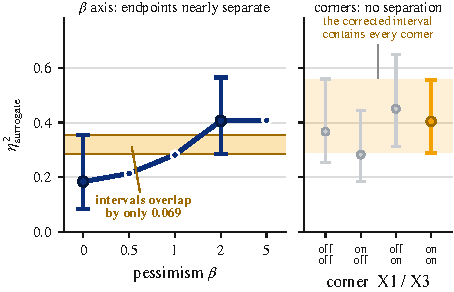
\includegraphics[width=0.99\columnwidth]{figures_v3/fig_beta_resolution}
\caption{$\beta$ nearly resolves where the engine corners do not. Left: $\eta^2_{\text{surr}}$ rises monotonically with pessimism, the $\beta{=}0$ and $\beta{=}2$ intervals overlapping by only $0.069$ (intervals drawn at those two endpoints only). Right, on the same scale: the four corner intervals overlap completely. Synthetic grid, 7 tasks, 30 seeds, $B{=}10{,}000$.}
\label{fig:beta}
\end{figure}

\begin{table}[t]
\centering
\caption{Four-corner decomposition (synthetic, 7 tasks, 30 seeds, $B{=}10{,}000$ bootstrap). X1 standardizes the ensemble's targets; X3 equalizes the candidate/oracle protocol. The intervals overlap heavily: corner differences are \emph{not} resolvable at $n{=}7$.}
\label{tab:corners}
\small
\setlength{\tabcolsep}{3.5pt}
\begin{tabular}{llccc}
\toprule
X1\,/\,X3 & $\eta^2_{\text{surr}}$ [95\% CI] & $\eta^2_{\text{opt}}$ & $\eta^2_{\text{inter}}$ & Friedman $p$ \\
\midrule
off / off & $0.367$ $[0.254,0.559]$ & $0.013$ & $0.165$ & $6.1\times10^{-5}$ \\
on\ \,/ off & $0.283$ $[0.186,0.444]$ & $0.036$ & $0.146$ & $1.7\times10^{-3}$ \\
off / on\ \, & $0.450$ $[0.312,0.649]$ & $0.006$ & $0.152$ & $4.1\times10^{-5}$ \\
on\ \,/ on\ \, & $\mathbf{0.405}$ $[0.290,0.556]$ & $0.005$ & $0.160$ & $8.1\times10^{-4}$ \\
\bottomrule
\end{tabular}
\end{table}

\paragraph{The interaction is the term the design exists to estimate.} The fourth column of Table~\ref{tab:corners} is the one a one-factor-at-a-time study cannot produce, and we report it rather than print it. $\eta^2_{\text{inter}}$ is $0.165$, $0.146$, $0.152$ and $0.160$ across the four corners, with bootstrap intervals $[0.107,0.260]$, $[0.088,0.249]$, $[0.094,0.230]$ and $[0.087,0.236]$: the interval excludes zero in all four, at four to thirty-three times the optimizer main effect. It survives the same bias correction the main effects need, at $0.134$--$0.156$. And it is the most stable quantity in this paper: its range across corners is $0.018$ against the headline's $0.167$, so the coordinate the headline is most sensitive to barely moves it.

Three things follow, and a fourth bounds them. First, this is what the crossed design buys: one-factor-at-a-time experimentation cannot estimate interactions at all, which is the standard argument for a factorial \citep{nist2012handbook,box1978statistics}, and it is why the closest two-axis precedent names the analysis and declines it \citep{moosbauer2022benchmarkdriven}. Second, it is the missing evidence for a claim we make elsewhere: a small $\eta^2_{\text{opt}}$ licenses ``optimizer choice explains little \mdemph{marginal} variance'' and never ``optimizer choice is arbitrary,'' and the interaction is why: optimizer choice has a small marginal effect and a substantial conditional one, four to thirty-three times larger. That pattern is textbook rather than anomalous: a factor can be the least important main effect while appearing in almost every significant interaction, and large interactions can obscure main effects \citep{nist2012handbook}. Third, we concede the precedent in its defensible form. Interaction reporting is routine inside the functional-ANOVA tradition this design descends from, which decomposes into main effects and pairwise interactions by construction \citep{hutter2014fanova}; what we find no instance of is an interaction reported and interpreted between \mdemph{surrogate model class} and \mdemph{search routine} as two independently manipulated pipeline components.

The bound is that this is an existence-and-ordering claim under a disclosed normalizer, not the stable quantity ``$0.15$.'' Recomputing the full decomposition across four corners and three normalizers (Table~\ref{tab:normrob}), $\eta^2_{\text{surr}}>\eta^2_{\text{opt}}$ holds in \mdemph{all twelve} combinations and $\eta^2_{\text{surr}}$ is largest in all twelve, so the headline ordering is untouched; the interaction exceeds the optimizer main effect in \mdemph{eleven} of twelve, by $1.1\times$ to $71.3\times$, and inverts in one, the on/off corner under rank normalization, which carries the largest optimizer main effect under every normalizer. Rank transformation roughly halves the interaction throughout. The second bound is suite-specific: on Design-Bench $\eta^2_{\text{inter}}$ is only $0.007$--$0.036$ and subordinate to $\eta^2_{\text{opt}}$ there, and we cannot explain the failure to generalize. Frozen cells are a candidate (a cell returning a bit-identical constant can carry neither a main effect nor an interaction), but Design-Bench's own $\eta^2_{\text{opt}}$ of $0.05$--$0.17$ shows the axes are not all flattened, so we state the scoping as an unexplained limit, not a resolved one.

\begin{table}[t]
\centering
\caption{Normalizer robustness. Four engine corners $\times$ three per-task normalizers, recomputed from the stored per-seed grids. $\eta^2_{\text{surr}}>\eta^2_{\text{opt}}$ in all twelve; $\eta^2_{\text{inter}}>\eta^2_{\text{opt}}$ in eleven, inverting only in the marked row.}
\label{tab:normrob}
\small
\setlength{\tabcolsep}{3.5pt}
\begin{tabular}{llcccr}
\toprule
Corner & Norm. & $\eta^2_{\text{surr}}$ & $\eta^2_{\text{opt}}$ & $\eta^2_{\text{inter}}$ & int/opt \\
\midrule
off / off & min--max & $0.367$ & $0.013$ & $0.165$ & $12.4\times$ \\
off / off & $z$-score & $0.426$ & $0.019$ & $0.193$ & $10.0\times$ \\
off / off & rank      & $0.487$ & $0.050$ & $0.053$ & $1.1\times$ \\
on\ \,/ off & min--max & $0.283$ & $0.036$ & $0.146$ & $4.0\times$ \\
on\ \,/ off & $z$-score & $0.347$ & $0.042$ & $0.189$ & $4.5\times$ \\
on\ \,/ off & rank     & $0.318$ & $0.075$ & $0.049$ & $\mathbf{0.6\times}$ \\
off / on\ \, & min--max & $0.450$ & $0.006$ & $0.152$ & $26.9\times$ \\
off / on\ \, & $z$-score & $0.494$ & $0.008$ & $0.167$ & $20.6\times$ \\
off / on\ \, & rank     & $0.524$ & $0.021$ & $0.062$ & $2.9\times$ \\
on\ \,/ on\ \, & min--max & $0.405$ & $0.005$ & $0.160$ & $32.8\times$ \\
on\ \,/ on\ \, & $z$-score & $0.454$ & $0.003$ & $0.179$ & $71.3\times$ \\
on\ \,/ on\ \, & rank     & $0.388$ & $0.017$ & $0.071$ & $4.1\times$ \\
\bottomrule
\end{tabular}
\end{table}

\section{Isolating the Source of the Gap}
\label{sec:mech}

We ran seven controls, each capable of explaining the GP--ensemble gap, and none does (Table~\ref{tab:elim}). Two were built to confirm accounts of our own and refuted them instead. Each control's scope travels with it, because a bare count of seven would claim more than two of them establish: capacity is eliminated at fixed depth, and $\sigma$ at this ensemble construction. Eliminations~1 ($\sigma$/pessimism) and~7 (the oracle-value localization) carry the section's weight and are developed below; the other five are Table~\ref{tab:elim}.

\begin{table}[t]
\centering
\caption{The seven controls on the GP--ensemble gap; none closes it (audited synthetic grid, $\beta{=}2$, $K{=}5$, 30 seeds). Eliminations~1 and~7 are developed in prose below; the middle five are stated here, with detail in the supplement. Elimination~2 supports that the gap \emph{does not close}, not that it is identical at $w{=}1024$ (its least precise point), and answers the width objection at practical widths only---the NTK limit is asymptotic, so the depth-driven form remains open.}
\label{tab:elim}
\footnotesize
\setlength{\tabcolsep}{3pt}
\begin{tabular}{@{}rl p{4.85cm}@{}}
\toprule
\# & Rules out & Decisive evidence \\
\midrule
1 & pessimism / $\sigma$ & $61\%$ of the advantage survives at $\beta{=}0$; cross-$\beta$ gap $0.319$ vs $0.525$ \emph{(prose)} \\
2 & finite width & gap flat over $10.7\times$ width, $0.480\!\to\!0.476$, $99.1\%$ retained (Supp.\ Fig.\ S2) \\
3 & predictive accuracy & ensemble RMSE below the GP's at every width; tie-cells $0.375$ (registered primary), $7/7$ tasks (post-hoc); still loses by ${\sim}0.48$; NLL is calibration (Supp.\ Fig.\ S2) \\
4 & search budget & more budget \emph{widens} the gap; ensemble marginal $0.361\!\to\!0.240$ while both GPs rise (observation, not pre-registered) \\
5 & mean roughness & roughness cut up to $98\%$ both ways, gap widened, no closing interval; GP-roughening arm void \\
6 & premise coverage & own-proposal coverage ${\to}0.998$, gap unmoved; $\rho(\text{cov},\text{score}){=}0.29$ \\
7 & distance / inflation & distance and inflation both null; loss real, $-1.406$ $[-2.803,-0.375]$ at matched distance \emph{(prose)} \\
\bottomrule
\end{tabular}
\end{table}

\paragraph{On our tasks, $\sigma$ tracks distance more than error.} The ensemble's $\sigma$ correlates with pointwise absolute error at only $\rho\approx0.07$ but with $k$-NN distance to the training data at $\rho\approx0.26$: three to four times larger, positive on all seven tasks, above $0.28$ on the four tasks between 5 and 15 dimensions (and $0.20$--$0.23$ at 20 and 30). The prior analysis concluded $\sigma$ was uninformative by measuring it against the wrong target; this is the corrected measurement. Read against the distance-aware literature it is a \mdemph{contrast}, not a corroboration: deep ensembles are exactly the class that work characterizes as \mdemph{not} distance aware, assigning low uncertainty far from the data \citep{liu2020sngp,vanamersfoort2020duq}, where ours shows a modest positive distance correlation. Two scope gaps keep that honest: those results validate on classification with no regression, and they measure geometry we do not reproduce.

One alternative for $\rho\approx0.07$ we did not examine and do not exclude: our $\sigma$ is the empirical standard deviation across $K$ squared-error members, the construction contrasted against a likelihood-trained heteroscedastic ensemble and reported to underestimate predictive uncertainty (an 80\% nominal interval covering roughly 20\% of observations) \citep{lakshminarayanan2017ensembles}. The low error correlation may therefore be a property of this construction, not of ensembles generally. We did not run the likelihood-trained variant, so Elimination~1 removes $\sigma$ \mdemph{as constructed here}; a different construction is an open arm. We do not claim squared-error ensembles are broken.

\paragraph{Elimination 1: it is not $\sigma$.} With pessimism removed entirely ($\beta{=}0$, pure posterior-mean maximization), $61\%$ of the GP's advantage survives and the interval excludes zero: the marginal gap is $0.319$ $[0.196,0.460]$ at $\beta{=}0$ against $0.525$ $[0.406,0.614]$ at $\beta{=}2$, both read on one $\beta$-invariant normalizer (a per-task min--max fit once over the pooled cell means of both conditions, refit inside each bootstrap resample). The pessimism increment is itself significant ($0.203$ $[0.007,0.396]$, $p{=}0.020$), so the statement is base-plus-amplification: pessimism \mdemph{amplifies} a mean-quality base rather than creating it, and any claim that the advantage is independent of pessimism is refuted by our own data. It passes narrowly: the surviving base of $0.319$ clears its pre-registered collapse threshold of $0.263$ by a margin inside the bootstrap interval. That increment is a paired bootstrap delta, resampled jointly, not a difference of marginals (subtracting the point estimates gives $0.206$). The cross-check is our strongest single evidence: recomputed on a per-task $z$-score, the same two conditions give $0.904$ against $1.473$ standard deviations, a ratio of $0.614$ against $0.608$ on the min--max scale, within $0.006$ on a different scale, which makes this a measurement, not a normalization artifact.

\paragraph{Elimination 7: it is not distance to the data, nor surrogate inflation.} The next hypothesis is that the ensemble's optima sit further off-support, where its mean is free to invent maxima, and that it over-predicts them more. We pre-registered both limbs and instrumented every returned optimum with its $10$-NN distance to the offline data and its over-prediction against the oracle ($168$ cells, $30$ seeds, bit-exact at seed~0). Both come back null: the ensemble's optima are $+0.116$ $[-0.004,0.333]$ further out and $+0.043$ $[-0.652,1.085]$ more inflated, both intervals covering zero, and the distance is one task (Branin-2D contributes $+0.743$, the other six lie between $-0.022$ and $+0.060$). The loss is not null: at those optima the ensemble is worse in \mdemph{true oracle value} by $-1.406$ $[-2.803,-0.375]$ in units of $\mathrm{sd}(y_\D)$, excluding zero, and worse in four of five distance bins, tied in the fifth. The landscape law behind those bins is real (across $5{,}040$ optima, distance predicts both over-prediction, $\rho{=}{+}0.758$, and true loss, $\rho{=}{-}0.818$) but does not discriminate (Figure~\ref{fig:landscape}): the classes sit at the same median distance ($0.87$ against $0.86$) and differ in outcome anyway. Off-support maxima are inflated and worthless, a property of the problem, not of the ensemble.

That law is not ours, and stating whose sharpens what we add. \citet{fannjiang2020autofocused} articulated it in 2020: oracle-based design queries the oracle where its training data does not reach, so its outputs, \mdemph{including its uncertainty estimates}, become unreliable off-support. Our measurement confirms that account in aggregate and shows it \mdemph{insufficient} for our question: off-support degradation is shared by every surrogate class here, so it cannot explain a difference \mdemph{between} classes, and at matched median distance ($0.87$ / $0.86$ / $0.84$) the ensemble is still worse in true oracle value by $-1.406$ $[-2.803,-0.375]$. The off-support story is right about where surrogates fail and silent about which maximizers each class admits once there. The same distance-graded degradation has a quantitative form elsewhere, where over-optimizing a learned proxy degrades true reward along closed-form curves whose coefficients depend on the proxy's class \citep{gao2023reward}; our Elimination~7 moves that shape onto a new axis, architecture class rather than model scale, rather than contradicting it.

\begin{figure*}[t]
\centering
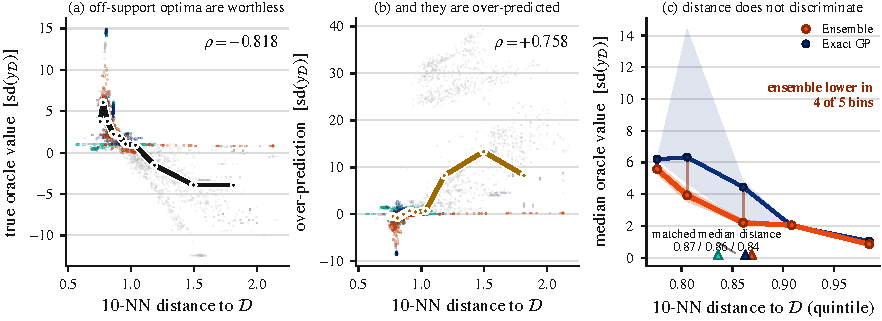
\includegraphics[width=0.99\textwidth]{figures_v3/fig_landscape}
\caption{Distance predicts both worthlessness (a, $\rho{=}{-}0.818$) and over-prediction (b, $\rho{=}{+}0.758$) across all $5{,}040$ returned optima, but does not discriminate between surrogate classes (c): they sit at matched median distance ($0.87$/$0.86$/$0.84$) and the ensemble is still lower in oracle value, in four of five bins. Panel~(c) compares the ensemble against the exact GP (SVGP omitted, its distance--value correlation near zero); bands are $95\%$ bootstrap intervals on the bin median. Audited engine, X1 and X3 on, $\beta{=}2$, $K{=}5$.}
\label{fig:landscape}
\end{figure*}

The second limb is uninformative rather than negative. It proposed raising the GP's prior mean until its far field stopped reverting to the data mean, but the manipulation does not move its target: a constant above every observation shifts the far-field posterior mean by under $1\%$ of the distance to it ($R{=}0.009$ against a registered $0.25$), because the fitted lengthscales are of order the domain diameter and no point in the feasible cube is in a reversion regime. The one arm that does remove reversion carries $211\times$ the incumbent's held-out RMSE, and a surrogate that has stopped predicting is not evidence about reversion. A premise failed rather than a prediction surviving, which establishes that any account of the GP's advantage resting on prior reversion is here unavailable, not merely untested.

\paragraph{The gap survives seven controls.} None of the seven survives (Table~\ref{tab:elim}); one, more search budget, corroborates the mean-geometry reading by making the ensemble relatively worse as both GPs convert budget into score. The seventh adds a positive localization: the loss is real and sits at the returned optimum's oracle quality, while every landscape property we can construct to explain it is matched between the classes. What differs is \mdemph{which} off-distribution maximizers a surrogate's mean admits, not how rough those means are, how far out the optima lie, or how much they over-predict. That is a diagnosis, not a mechanism with a positive causal test, and we label it so. A skeptic could read this localization and Section~\ref{sec:deconf}'s interaction as one phenomenon counted twice: the ensemble's bad basins are reachable by gradient ascent and missed by perturbation, which \mdemph{is} the interaction. But these surrogate-geometry measurements do not read off the optimizer axis: the $\sigma$-against-distance correlation is a property of the surrogate alone, and the matched-distance oracle-value gap is pooled across all optimizers, whereas the interaction is a surrogate$\times$optimizer decomposition. The mechanism is one phenomenon triangulated by two independent instruments, an optimizer-agnostic geometry measurement and a factorial decomposition, not the interaction restated.

\paragraph{A question the grid poses and we test: is the advantage conditional on the optimizer?} The interaction says the surrogate gap depends on which optimizer is paired with it. In raw oracle units (no normalization, no bootstrap, so neither the normalizer critique nor the small-$n$ $\eta^2$ bias reaches this) the exact-GP--ensemble gap is smaller under perturbation than under \mdemph{both} gradient ascent and CMA on all seven tasks, spanning 2D to 30D, averaging under a tenth of the aggressive-optimizer gap; on Ackley-20D it closes entirely. We report this as a question, not a result, because the obvious competing explanation is not excluded and our one discriminating test points toward it. A floor effect (perturbation underperforming and compressing all three surrogate cells toward a common achievable value) would produce the same shape. The discriminating case is Styblinski-5D, the one task where perturbation is the grid's \mdemph{best} optimizer (GP with perturbation at $35.9$), and it carries by far the \mdemph{weakest} attenuation, $40\%$ of the aggressive gap against at most $8.8\%$ elsewhere: what a floor effect predicts, not what a genuine neutralization predicts. One contrary point at $n{=}7$ does not settle it, but it is the only case that speaks to it and it speaks against the causal reading. The descriptive fact is solid; the mechanism is not. Ensembles paired with gradient ascent produced systematic inversions (Figure~\ref{fig:x0}) while perturbation attenuated the gap; whether that is a genuine surrogate$\times$optimizer interaction or the floor effect is unresolved.

\paragraph{The acquisition ranks its own hallucinations above designs it holds.} What ``admits an off-distribution maximizer'' costs is measurable directly, because the candidate/oracle correction puts the starting designs \mdemph{inside} the returned pool: every cell is seeded with the top-128 offline designs plus lightly perturbed copies, and gradient and perturbation optimizers pool every iterate with that seed set before returning the top 128 by surrogate LCB. A cell returning something worse than what it was handed has had its acquisition rank an invented design above a real one it was holding. We call that an inversion and count it per seed (Figure~\ref{fig:x0}). It is close to ensemble-specific: on the audited engine the ensemble inverts on at least one optimizer on all seven tasks, against three of seven for the SVGP and two for the exact GP, and where the GPs invert they do so on tasks the ensemble inverts on more heavily. The sharpest cell is Branin-2D under ensemble gradient ascent (six other ensemble and SVGP cells tie it, seven in all at unit inversion rate and unit mean fraction worse), where all 30 seeds invert and \mdemph{every one} of the 128 returned designs scores below the best design the cell started with. This is the elimination-7 localization made concrete: the loss sits at the returned optimum's oracle quality; a demonstration within this grid, descriptive at $n{=}7$ tasks, not a mechanism with a causal test behind it.

What it is an instance of has a name. Offline RL formalizes the requirement that a policy learned from a fixed dataset not be worse than the baseline it was given, with high probability, as \mdemph{safe policy improvement}, and measures algorithms by how often they violate it \citep{thomas2015hcpi,laroche2019spibb}; the conservative-value lineage supplies the complementary shape, the learned value function widening rather than inverting the gap between in-distribution and off-support designs \citep{kumar2020cql}. Offline MBO optimizers ship no analogous guarantee, and the inversion is what that absence looks like measured: an acquisition returning designs worse than the ones it was handed is a safe-improvement failure, not merely an awkward number.


\begin{figure*}[t]
\centering
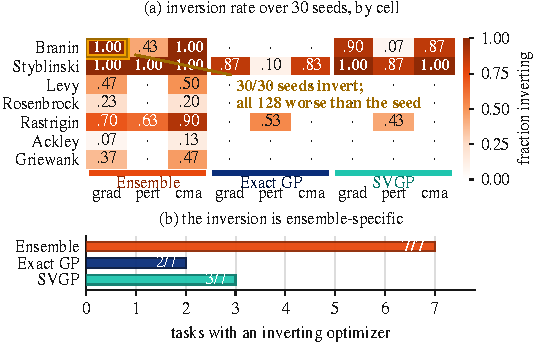
\includegraphics[width=0.99\textwidth]{figures_v3/fig_x0_inversion}
\caption{The ensemble's LCB ranks designs it invented above real designs it was handed. (a)~Inversion rate over 30 seeds for all 63 cells: the ensemble block lights up, the exact GP's stays dark. (b)~Tasks with at least one inverting optimizer: 7/7 ensemble, 3/7 SVGP, 2/7 exact GP. Audited engine, X1 and X3 on, $K{=}5$, $\beta{=}2$, 30 seeds.}
\label{fig:x0}
\end{figure*}

\paragraph{Gradient collapse on the audited engine.} Our own released tuning sweep concluded that the ensemble's gradient collapse is an artifact a trust region repairs, a result absent from the prior analysis. We report it in full, including the corner where it fires against us. By the sweep's own $5\%$ rule, the tasks whose collapse survives tuning number $2/7$ with neither correction, $0/7$ under target scaling alone, $5/7$ under the protocol correction alone, and $4/7$ on the audited engine. The collapse is genuine surrogate geometry on most tasks, driven by the candidate/oracle correction rather than target scaling, and on one corner not genuine at all.

\paragraph{Two corrections to the coverage analysis.} First, the collapse is not gradient-specific. We registered that ensemble coverage would also be low on CMA proposals; it is. Under the matched protocol gradient and CMA proposals differ in out-of-distribution coverage by $0.010$, against $0.117$ under the unmatched one, because both pool every iterate and return the top 128 by surrogate LCB. The claim narrows to the ensemble paired with any aggressive selector, and we withdraw the gradient-specific framing by name. Second, the premise-coverage value of $0.97$ in the prior analysis belongs to a scikit-learn exact GP, not the differentiable GP the grid scores, whose coverage averages $0.831$ and falls to $0.38$ on Styblinski-5D; both are reported with the model each belongs to. Coverage of $\{\mu-f\le\beta\sigma\}$ is exactly the validity of the lower bound, which is what makes these frequencies worth measuring.

\section{Design-Bench Results}
\label{sec:db}

\paragraph{The surrogate null.} Across all four engine corners the Design-Bench surrogate main effect is essentially zero ($\eta^2_{\text{surr}}$ of $0.001$--$0.032$ on five tasks, every estimate at the floor of its bootstrap interval) and the Friedman omnibus fails to reject ($p = 0.19$ to $0.76$). We report no detectable difference at this power, never equivalence: at $n{=}7$ a paired test needs $|d_z|\geq1.27$ for $80\%$ power, larger than anything we observe, and a failure to reject does not demonstrate absence \citep{agarwal2021precipice}. The null is not fragile to the task set. Dropping GFP leaves it ($\eta^2_{\text{surr}}$ $0.001$--$0.021$); adding the two MuJoCo tasks makes the omnibus reject in three of four corners but does \mdemph{not} lift $\eta^2_{\text{surr}}$ off the floor: it rises only to $0.044$--$0.091$, still four to nine times below the synthetic grid's $0.405$, while the optimizer effect runs $1.6$ to $4.5\times$ larger and the one non-rejecting corner carries the \mdemph{larger} surrogate effect ($0.053$ against a rejecting corner's $0.044$). Surrogate size does not track rejection; the optimizer axis does, which is why we report the rejection under its own decomposition rather than dropping the tasks that produce it. The null also survives the exact-oracle subset in every corner ($p = 0.34$ to $0.51$), so it is not manufactured by approximate oracles, and repeated oracle evaluation is noiseless to machine precision, so the null is not noise drowning a signal; with two exact-oracle tasks that subset test is low-powered, so this is consistency with the null, not a powered acceptance (supplement). A prior pooling defect---eleven cells, two undefined---is unified to the nine defined cells before any rank claim, since mean ranks depend on the pool \citep{benavoli2016meanranks}.

\paragraph{Matching the query budget strengthens the optimizer axis.} Everything above is at native budgets, where gradient outspends perturbation by $6.25\times$ (X3-off) to $11.8\times$ (X3-on), so the optimizer axis could be search intensity in a costume. Equalizing surrogate queries across the full seven-task grid (at $Q{=}25{,}600$ and $51{,}456$; none of 252 cells over $5\%$ off target) runs \mdemph{backwards} to that objection: matching does not shrink the optimizer effect but raises it $1.46$ to $1.88\times$ in every corner ($\eta^2_{\text{opt}}$ $0.096\!\to\!0.180$, $0.145\!\to\!0.255$, $0.193\!\to\!0.282$, $0.181\!\to\!0.281$) while $\eta^2_{\text{surr}}$ \mdemph{falls} in all four, and it flips off\_off into rejection, so under matched budgets \mdemph{all four} corners reject ($p = 0.0179$ to $0.00057$) where three did. The native imbalance was \mdemph{masking} the optimizer effect, not manufacturing it. Two scope limits are ours: this is \mdemph{established at high budget}---at the matched low level $\eta^2_{\text{surr}}$ reaches $0.126$, above our $0.10$ floor, and one corner ties ($\eta^2_{\text{opt}}$ $0.085$ against $\eta^2_{\text{surr}}$ $0.081$), so the pre-registered primary level decides---and the within-corner intervals overlap, so what is licensed is point-estimate localization across corners. The ``all four reject'' count is the seven-task set; the five-task and GFP-dropped sets reject three of four under matching, in the same direction. A native-budget control through the matched runner reproduces the published corners to within $0.004$ on every $\eta^2$, so the contrast is budget, not call order.

\paragraph{Frozen cells are a benchmark-construction finding.} Part of the null is structural, and a reusable result in its own right: several of Design-Bench's cells are degenerate for surrogate attribution, freezing at the dataset reference so they carry neither a main effect nor an interaction. On TF-Bind-8 the three exact-GP cells return exactly $1.0$ on all 16 seeds with zero variance, and ensemble-with-perturbation joins them in two corners---up to four frozen cells of nine---where $1.0$ is not a score but the min--max-normalized dataset maximum, already attained by tied rows, so the cell returned nothing better than its input. On Ant, two of three GP cells return the bit-identical constant $1.5287419557571411$ with standard deviation exactly $0.0$ across all sixteen seeds, and a third (SVGP with perturbation) on ten of sixteen: three cells across two surrogate classes converging on one value is retrieval, not coincidence. An attribution study here must screen for frozen cells first, or read a surrogate axis that cannot move as evidence about surrogates. The mechanism is \mdemph{LCB paralysis}, not decode snap-back: decode snap-back predicts that an exact-constant freeze needs a decode step, but Ant is continuous with no argmax decode, so our pre-registered kill against it fires, and the GP's lower confidence bound is simply locally maximal at the data, with sixteen bit-identical seeds across two GP implementations as our own evidence. The nearest prior formalization is an inconsistency result for expected-improvement BO \citep{yarotsky2013inconsistency}, differing on three axes (expected improvement not a confidence bound, online not offline, adversarial not seed-robust); the trust-region literature uses the same locality \mdemph{deliberately} \citep{eriksson2019turbo} where here it is an unintended terminal state. This does not rescue our own positive signal, which stays synthetic-only.

\paragraph{The inversion and the synthetic null are one finding.} The section's most awkward number is that the optimizer axis \mdemph{inverts} here---perturbation leads all four corners ($0.76$--$0.81$ against gradient's $0.40$--$0.68$), $\eta^2_{\text{opt}}$ exceeding $\eta^2_{\text{surr}}$ in point estimate everywhere (intervals overlap, so this is point-estimate localization, never a within-corner separation)---while the synthetic optimizer effect is small ($\eta^2_{\text{opt}}{=}0.038$ $[0.003,0.123]$ under matched budgets, a magnitude for that grid, not a verdict that optimizer choice is negligible in general; Section~\ref{sec:limits}). Read through the frozen cells the two suites stop disagreeing: if the GP cannot be moved, every optimizer scores it identically, the surviving between-optimizer variance comes from the unfrozen ensemble cells, and the axis inverts as an arithmetic consequence of the freeze, not a contradiction between benchmarks---the payoff of a decomposition over a leaderboard. Four limits: it is two of three Ant GP cells, not three (the gradient cell returns $1.3242 \pm 0.1975$, unfrozen); fact and label are separable; frozen and genuinely near-tied cells are never pooled; and the freeze explains why the axis inverts, not how large the optimizer effect is, which the matched-budget arm establishes.

\section{Discussion and Limitations}
\label{sec:limits}

\paragraph{Pre-registered predictions and their outcomes.} Four registered predictions came back against us and two registered mechanism arms failed to deliver what they were built for; we report all six, because undisclosed they would read as selective reporting to anyone who opens the repository. Our registered headline was that the acquisition optimizer explains most of the reported gap: in this grid it does not, $\eta^2_{\text{opt}}$ being $0.038$ even after correcting the budget imbalance that suppressed it, and the pre-committed contingency (pivot to the mechanism rather than quietly restate) is what this paper does. The ensemble-size reversal criterion did not fire, but its accompanying prediction confirmed: the headline is reported at the $K$ that maximizes it (Confound~3). The $\beta$--$\sigma$ criterion fired outright, narrowing Confound~4 to its per-task form, and the gradient-specific coverage framing was retracted on our own registered test. The two mechanism arms are the most expensive: smoothing the ensemble's mean was built to confirm the account we had published and refuted it, and the phantom-maxima probe was built to establish a mechanism and returned a seventh elimination.

\paragraph{Interpreting the optimizer effect.} Under a matched surrogate-query budget of $Q{=}51{,}456$, $\eta^2_{\text{opt}} = 0.038$ $[0.003,0.123]$, so optimizer choice explains little of the variance in this grid. Three qualifications travel with it. It replaces our own unmatched $0.005$ that understates by roughly eightfold, a correction we disclose. The confirmation is not comfortable: the upper bound of $0.123$ lies inside our pre-registered inconclusive band, so an effect up to about $0.12$ is not excluded at $n{=}7$, the same precision limit that makes the corner decomposition unresolvable. And the secondary budget level does not corroborate cleanly ($0.066$ $[0.014,0.340]$ at $Q{=}4{,}352$), so the null is established at high budget and underpowered at low, never unqualified. Most importantly, the \mdemph{best} optimizer changes with budget: gradient leads at low budget ($0.731$) and perturbation at high ($0.732$), where the unmatched grid showed gradient modestly best throughout, an $11.8\times$ imbalance hiding itself by making one optimizer look mildly best everywhere. As Section~\ref{sec:deconf} measures, the small \mdemph{marginal} is not a verdict that optimizer choice is arbitrary: its \mdemph{conditional} effect through the interaction is four to thirty-three times larger, so which optimizer to use depends on the surrogate, the one thing a factorial and not a one-factor-at-a-time design can say.

\paragraph{Two confounds whose removal strengthens what they were meant to explain.} The synthetic and Design-Bench budget arms now make the same shape of finding on two independent axes. Correcting the protocol confounds raised the surrogate main effect on the synthetic grid from our decomposition of PGS's Table 1 ($\eta^2_{\text{surr}}\approx0.37$) \citep{chemingui2024pggs} to $0.405$ $[0.290,0.556]$; equalizing query budgets on Design-Bench raised the optimizer main effect by half again to nearly double in every corner rather than dissolving it. In both cases the confound was suppressing the effect it was suspected of manufacturing, and in both cases the direction runs against the reality-check genre's, where corrected effects shrink \citep{melis2018sota}. We state the limit of that pattern as plainly as the pattern. It is two instances, not a law: the ensemble-size confound moves the surrogate effect the other way (Confound~3), so we claim neither that de-confounding generally strengthens nor that these two corrections share a mechanism. What they share is that a reviewer's prior about which way a control will move is not evidence about which way it moved, and both of ours were measured rather than assumed. The pattern survives bias correction and grows slightly under it: $\eta^2$ is positively biased at small $n$, and our own bootstrap artifacts put that bias at $+0.0099$ to $+0.0184$ across the four corners. Bias-correcting the two-confound comparison gives $0.351\to0.395$, an increment of $+0.0437$ against the $+0.0376$ of the uncorrected figures. We report $\epsilon^2$ rather than $\omega^2$ as the correction, on simulation evidence naming $\epsilon^2$ the least-biased of the standard indices rather than the folk preference for $\omega^2$ \citep{okada2013epsilon}.

\paragraph{No landscape covariate we tested predicts the gap.} A natural objection is that the surrogate gap is really a landscape property in disguise. We tested every covariate we can construct and none predicts it at this power. The gap's rank correlation with dimension is $+0.107$ under gradient, $+0.036$ under perturbation and $+0.071$ under CMA, indistinguishable from zero under every optimizer ($p\geq0.81$), and pointing opposite the qualitative expectation that GP advantage should decay with dimension as neural surrogates learn non-stationarity that GPs need human intervention to capture \citep{li2024bnnsurrogates}. That is a measured refinement of a named prior expectation, not a disagreement about anything either of us tested directly. Textbook multimodality actively mis-sorts: within the ``many local minima'' family the gap spans three orders of magnitude, while the one strictly unimodal task has among the smallest gaps. Separability fares no better. This is a null from looking rather than from failing to look, and not an artifact of a flattening reparametrization: each task is mapped from the shared unit cube back onto its exact native textbook domain.

One structural statement does survive, and we weight it honestly. The per-task gap \mdemph{ordering} is stable across optimizers (Spearman $0.71$--$0.96$; the gradient-versus-perturbation pair at $0.71$ does not reach significance at $n{=}7$, $p{=}0.07$) while the gap \mdemph{magnitude} collapses under perturbation. Those are not in tension (one is relative ordering across tasks, the other absolute magnitude within an optimizer), and together they constrain any surviving mechanism to be multiplicative, a task factor scaled by an optimizer-aggressiveness factor. The collapse is bootstrapped; the ordering stability is descriptive at $n{=}7$, so the collapse is the better-evidenced half and the multiplicative reading is a constraint on future accounts rather than an account.

\paragraph{What the null does and does not license.} We never claim equivalence on Design-Bench, and we can say more than that disclaimer. The released code computes a paired two-one-sided-tests bound, which we report rather than withhold: the best-versus-worst gap is $0.376$ with a 90\% interval of $[-0.108,0.860]$ and an effect bound of $0.484$, which is \mdemph{not} equivalent at either a $0.5$ or a $0.3$ margin \citep{lakens2017equivalence}. So the null is a failure to detect that also fails to bound the effect below a margin anyone would call negligible, and rejecting small effects would require samples we do not have. That is a positive statement about the null's reach and it is weaker than equivalence in the direction that matters.

\paragraph{Robustness of the decomposition to its normalizer.} Because the per-task normalizer is an operating-point coordinate rather than a neutral choice, we recomputed the decomposition under $z$-score and rank transformations in every corner (Table~\ref{tab:normrob}), and under leave-one-task-out. Every combination preserves $\eta^2_{\text{surr}}>\eta^2_{\text{opt}}$; magnitudes move and the interaction roughly halves under rank, but the direction does not. Leave-one-task-out moves the headline between $0.373$ and $0.485$, and we correct one expectation of our own: Griewank-30D, whose raw score range is by far the widest and which we had flagged as the likely dominant lever, is the \mdemph{smallest} one, dropping it moving $0.405$ to $0.395$ while dropping Styblinski-5D moves it to $0.485$.

\paragraph{Scope of the optimizer-axis claim.} We make no field-reversal claim. That the choice of statistical model often matters more than the acquisition heuristic is the organizing doctrine of the standard Bayesian-optimization review \citep{shahriari2016humanoutoftheloop} and is a decade old; it governs online BO and the choice of acquisition \mdemph{function family}, not the numerical search routine in the offline setting. What our design falsifies is the local premise of one recent paper---that offline black-box optimization has focused on improving surrogate models while using fixed search strategies \citep{chemingui2024pggs}---by holding one shared protocol and varying both axes. We make no claim about the field's general beliefs about surrogates versus acquisitions. Nor do we claim ensemble size as a discovered mechanism \citep{li2024bnnsurrogates,abe2022ensembles}, equivalence on Design-Bench \citep{agarwal2021precipice,lakens2017equivalence}, priority on the $K$ range \citep{li2024bnnsurrogates}, or distance-aware uncertainty as ours \citep{liu2020sngp,vanamersfoort2020duq}.

\paragraph{Limitations.} Seven synthetic tasks is a small $n$, binding the corner decomposition, the optimizer interval and the Design-Bench omnibus alike. The synthetic datasets are drawn once at seed 0, so reported variance is training and optimization variance, not data-draw variance. GFP is quarantined from coverage claims because its decode is degenerate, and we report that both ways: excluding it, one claim flips (the exact GP's mean in-distribution coverage moves from below nominal to above it) while the effect-size null is unchanged. Budget matching now covers both suites, which lets Section~\ref{sec:db} assert its optimizer result rather than qualify it; what stays conditional there is the budget \mdemph{level}, since both the optimizer effect and the surrogate null weaken at the matched low budget. Two of the seven controls are narrower than the count suggests: capacity is eliminated at fixed depth 2, leaving the depth-driven form of that objection open, and $\sigma$ is eliminated at one ensemble construction, leaving a likelihood-trained variant untested. What the eliminations leave open is finite and namable---those two arms, plus whether the surrogate-geometry account and the optimizer interaction are one mechanism or two---so the argument bounds the residual rather than ranging over an open space. And the surviving mechanism statement is a diagnosis with seven eliminations behind it and no positive causal test in front: both positive accounts we pre-registered returned eliminations, not mechanisms. Off-support phantom maxima under prior reversion was refuted on its first limb and untestable on its second, the GP nowhere in a reversion regime inside the feasible set; and a far-field probe found the ensemble extrapolating near-linearly on all seven tasks while neither GP class reverts anywhere in the probed range, so far-field functional form does not distinguish the classes. Section~\ref{sec:mech} therefore ships as seven eliminations and a diagnosis, which is what the pre-registered binary licenses.

\section{Conclusion}

The reported advantage of GP-LCB in offline MBO is measured through five confounds specific to this comparison. Removing the two protocol confounds moves the surrogate main effect from our decomposition of PGS's Table 1 ($\eta^2_{\text{surr}}\approx0.37$) \citep{chemingui2024pggs} to $0.405$ $[0.290,0.556]$: against the direction every named audit in this genre ran, with no precedent we could find, and itself the net of two corrections against a third. That level is not resolvable at seven tasks, and we say so. Two firmer results remain. Any $\eta^2_{\text{surrogate}}$ here is a joint artifact of five operating-point coordinates papers do not state; and the surrogate$\times$optimizer interaction---the term this design exists to estimate, and a one-factor-at-a-time study cannot---exceeds the optimizer main effect in every corner, its interval excluding zero in all four. What the advantage \mdemph{is} remains open, narrowed by seven controls but not closed: not $\sigma$, width, budget, held-out accuracy, mean roughness, premise coverage, or distance-to-support with surrogate inflation. What is measured is the loss---the ensemble's optima worse in true oracle value at matched distance and matched inflation---and its shape, an acquisition ranking invented designs above real ones it was holding. On the optimizer axis the claim is narrow and stays narrow: under matched budgets $\eta^2_{\text{opt}}{=}0.038$ $[0.003,0.123]$ \mdemph{in this grid}, falsifying the local premise of one recent paper \citep{chemingui2024pggs} and claiming nothing about the field's general beliefs, which the standard review settled a decade ago \citep{shahriari2016humanoutoftheloop}. What we offer is the taxonomy, the protocol, and the engine stamp that makes either reproducible.

\section*{Ethical Statement}
This work studies optimization methodology on public benchmarks and introduces no new data or deployed system.

\bibliography{references}

\end{document}
